%!TEX root = ../../thesis.tex

\chapter{Related Work}
\label{rw:related_work}

This section reviews the pertinent literature relevant to the optimisation of CityJSON for cloud-native environments.

It highlights advancements and identifies existing gaps that this research aims to address.

\section{Cloud-Optimised Geospatial Formats}
\label{rw:cloud_optimised_formats}

Cloud-optimised geospatial formats constitute specialised data structures engineered to maximise computational efficiency in distributed cloud environments \citep{cloud-optimised-formats}.
These formats exhibit several quantifiable advantages:

\begin{itemize}
  \item \textbf{Reduced Latency}: Facilitates partial data retrieval and processing without necessitating complete file downloads.
  \item \textbf{Scalability}: Supports parallel operations through metadata-driven access mechanisms within cloud storage systems.
  \item \textbf{Flexibility}: Offers advanced query capabilities for selective data access.
  \item \textbf{Cost-Effectiveness}: Optimises storage and transfer expenditures through efficient access patterns.
\end{itemize}

\citet{cloud-optimised-formats} provides a comprehensive overview of several cloud-optimised geospatial formats.
These include Cloud Optimized GeoTIFF, Cloud Optimized Point Cloud, GeoParquet, PMTiles, FlatGeobuf.

\section{CityGML, CityJSON and Its Enhancements}
\label{rw:cityjson_enhancements}

\subsection{CityGML}
\label{rw:citygml}
CityGML is an OGC standard \citep{CityGML} that defines a comprehensive data model for representing 3D city models. The standard encompasses both geometric properties and rich semantic information through a modular structure. From version 3.0.0, CityGML separates its conceptual model from its encoding standard. Figure \autoref{fig:citygml_modules} shows an overview of its modules. The conceptual model defines the semantics and data model through a Core module and eleven thematic extension modules (Building, Bridge, Tunnel, Construction, CityFurniture, CityObjectGroup, LandUse, Relief, Transportation, Vegetation, and WaterBody). Additionally, five extension modules (Appearance, PointCloud, Generics, Versioning, and Dynamizer) provide specialized modeling capabilities applicable across all thematic modules. The encoding standard uses GML application schema for the Geography Markup Language (GML) \citep{gml} to encode the data. This modular design allows implementations to support specific subsets of modules based on their application requirements, ensuring flexibility while maintaining standard compliance.

\begin{figure}[htbp]
  \centering
  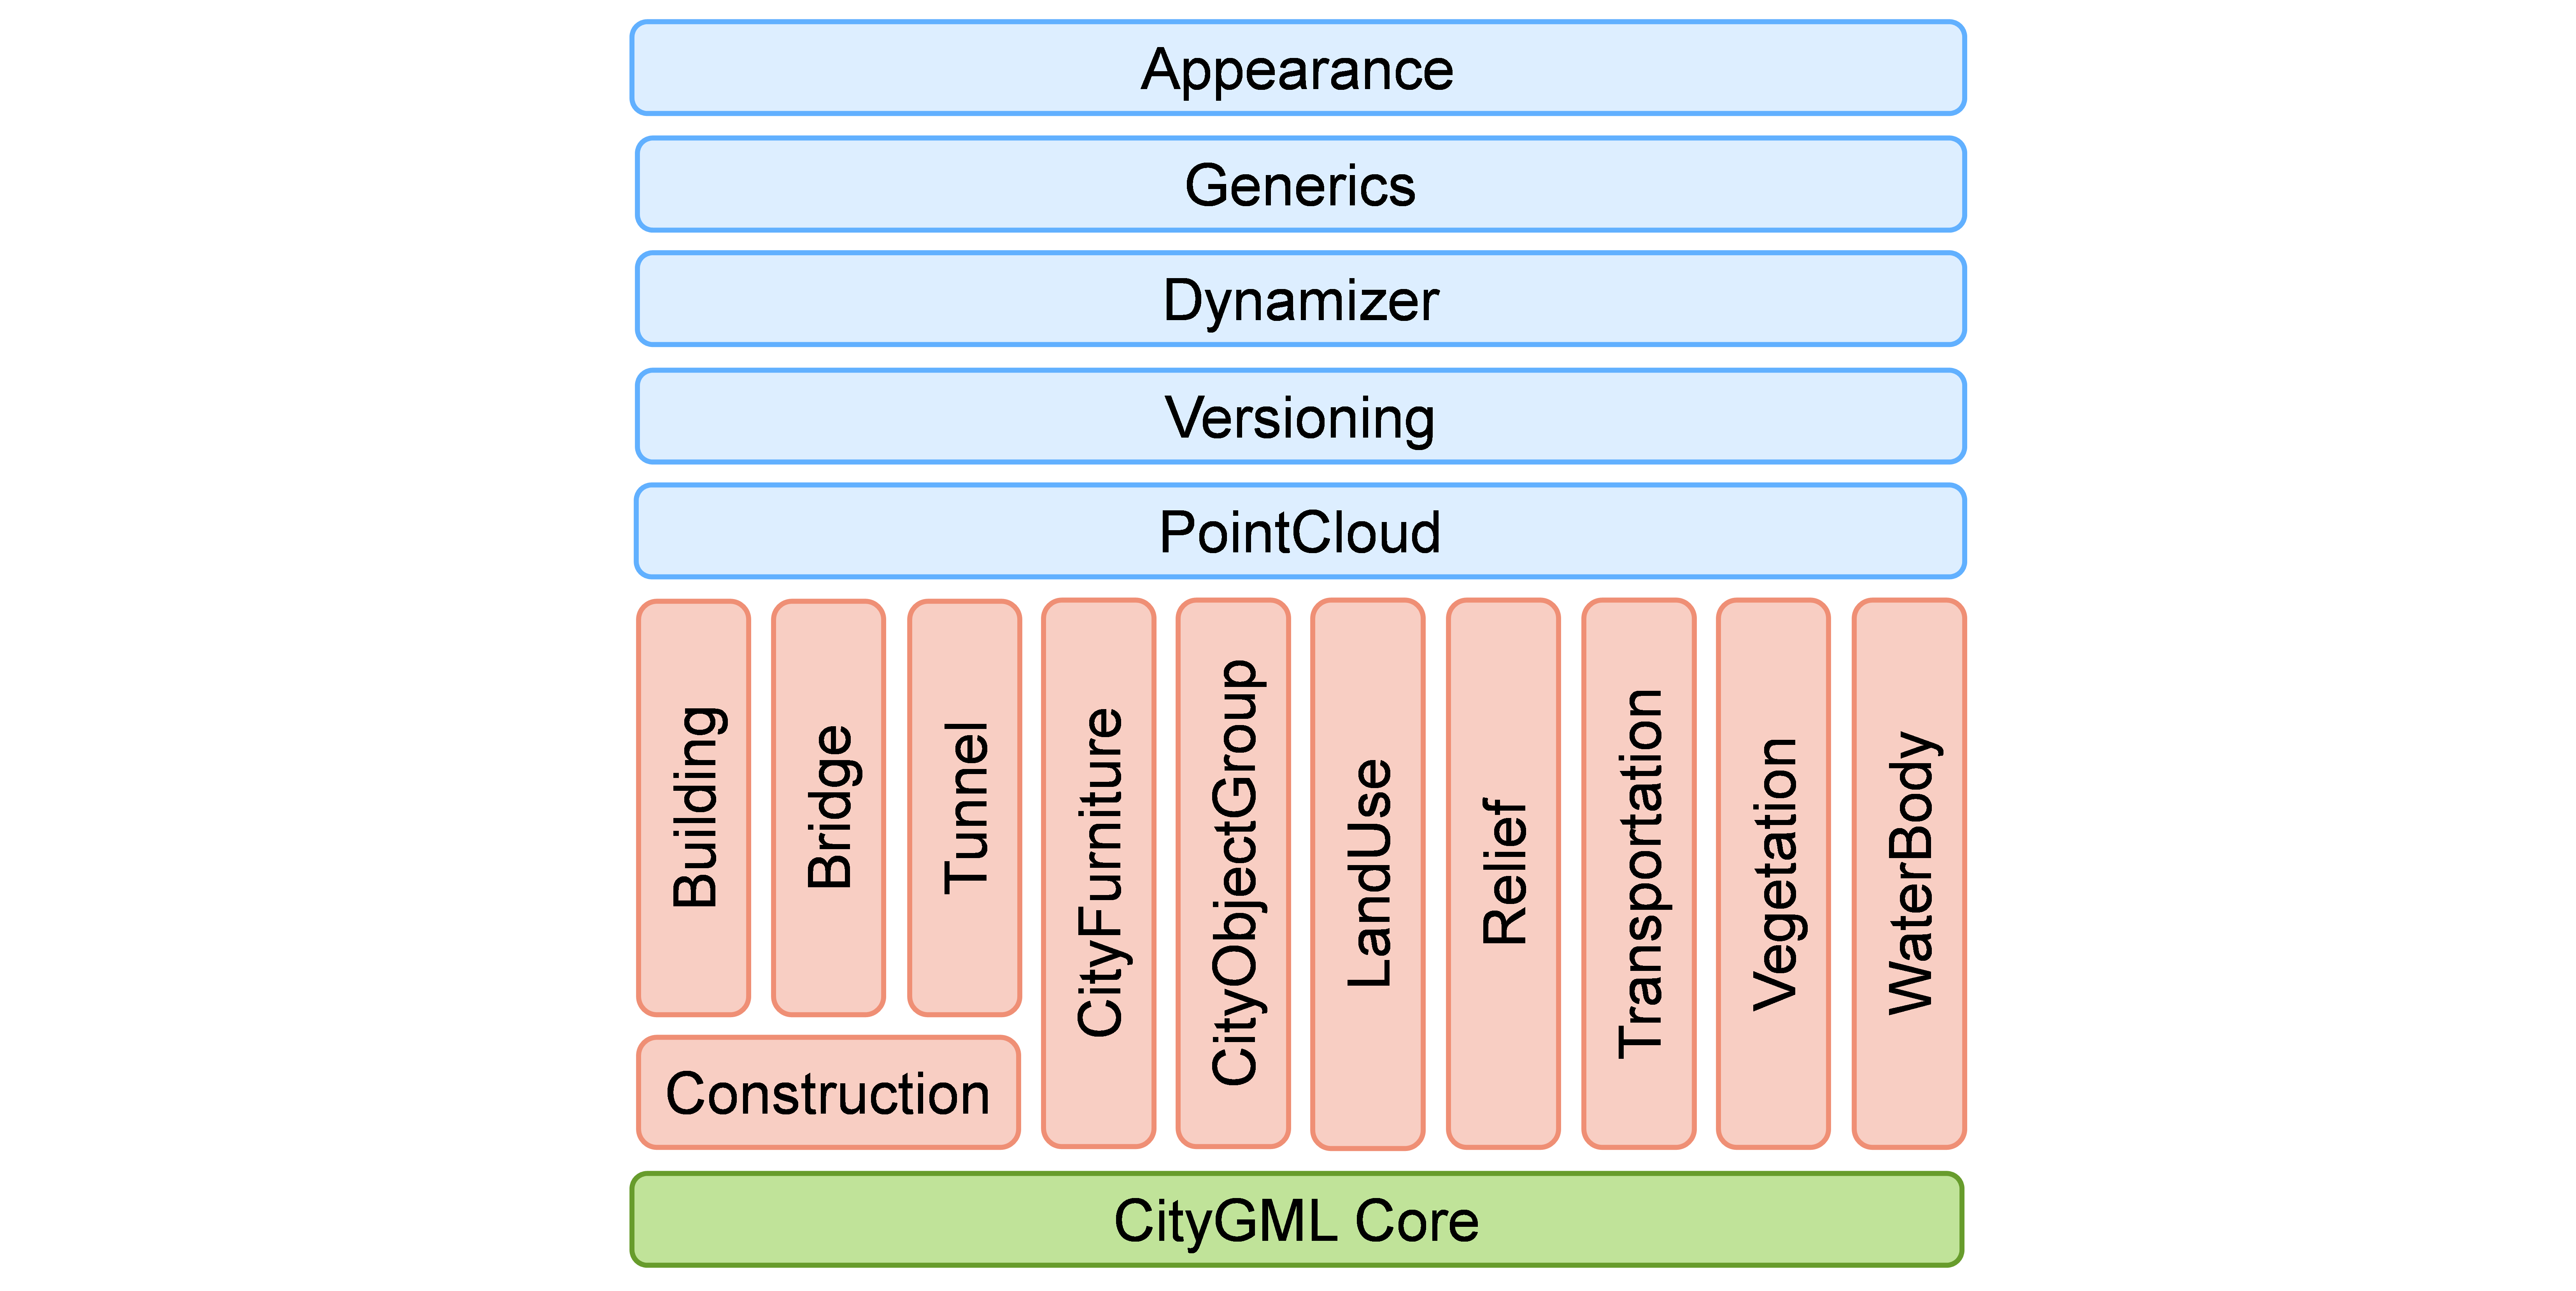
\includegraphics[width=0.8\textwidth]{figs/related_work_theoretical_bg/citygml3modules.png}
  \caption[CityGML 3.0 Module Overview]{Overview of CityGML 3.0 modules showing the Core module, thematic extension modules, and additional extension modules. Source: \citep{CityGML}}
  \label{fig:citygml_modules}
\end{figure}

\subsection{CityJSON}
\label{rw:cityjson}

CityJSON is a JSON-based \citep{json} encoding format that implements a subset of the CityGML conceptual model \citep{CityGML}. It is an official OGC standard \citep{ogc} currently at version 2.0.1, supporting CityGML 3.0.0 encoding. While both CityGML and CityJSON implement the CityGML conceptual model, CityJSON exhibits several notable differences.

The following properties of CityJSON are derived from \citet{ledoux_2019}:

\subsubsection{Flattened City Objects Architecture}
\label{rw:cityjson:flattened_architecture}

CityJSON implements a flattened architecture where each city object receives a unique identifier, contrasting with CityGML's hierarchical structure. While CityGML maintains a hierarchical organization, CityJSON stores all objects at the same level (e.g., first and second-level city objects are stored in the same dictionary). To preserve hierarchical relationships, CityJSON uses a \texttt{parents} field to reference each object's parent.

\subsubsection{Geometry}
\label{rw:cityjson:geometry}

CityJSON supports the same 3D geometric primitives as CityGML. However, instead of storing vertex coordinates directly within geometric primitives, CityJSON maintains a separate \texttt{vertices} array containing all coordinates. Geometric primitives then reference vertex positions within this array.

\subsubsection{Semantic Surfaces}
\label{rw:cityjson:semantic_surfaces}

CityJSON stores semantic surfaces as separate objects, recognizing that city objects often share common semantics. This is implemented through \texttt{semanticSurfaces} fields and a \texttt{values} array that maps surfaces to their corresponding semantic surface objects.

This is an example of how the semantic surfaces look like (derived from \citet{ledoux_2019}):

\begin{lstlisting}
  {
    "type": "Solid",
    "lod": 2,
    "boundaries": [
      [ [[0,3,2,1,22]], [[4,5,6,7]], [[0,1,5,4]],
        [[1,2,6,5]] ]
      ],
      "semantics": {
        "surfaces" : [
          { "type": "RoofSurface" },
          {
            "type": "WallSurface",
            "paint": "blue"
          },
          { "type": "GroundSurface" }
        ],
        "values": [ [0, 1, 1, 2] ]
      }
    }
  }
\end{lstlisting}

\subsubsection{Geometry Templates}
\label{rw:cityjson:geometry_templates}

CityJSON implements CityGML's Implicit Geometry concept through "geometry templates." The format includes \texttt{geometry-templates} fields with a \texttt{templates} array that stores reusable geometries. City objects utilizing these templates specify \texttt{"GeometryInstance"} in their geometry's \texttt{type} field to indicate template reuse.

This code shows an example of a geometry template derived from \citet{ledoux_2019}:

\begin{lstlisting}
  {
    "geometry-templates": {
      "templates": [{
        "type": "MultiSurface",
        "lod": 2,
        "boundaries": [
          [[0, 3, 2, 1]],
          [[4, 5, 6, 7]],
          [[0, 1, 5, 4]]
        ]
      }],
      "vertices-templates": [...]
    }
  }
\end{lstlisting}

And this is how a city object references this template:

\begin{lstlisting}
  {
    "type": "SolitaryVegetationObject",
    "geometry": [
      {
        "type": "GeometryInstance",
        "template": 0,
        "boundaries": [372],
        "transformationMatrix": [
          2.0, 0.0, 0.0, 0.0,
          0.0, 2.0, 0.0, 0.0,
          0.0, 0.0, 2.0, 0.0,
          0.0, 0.0, 0.0, 1.0
        ]
      }
    ]
  }
\end{lstlisting}

\subsubsection{Coordinate Quantization}
\label{rw:cityjson:coordinate_quantisation}

CityJSON employs coordinate quantization to reduce geometry size. The \texttt{transform} field contains \texttt{scale} and \texttt{translate} values for coordinate quantization. The original coordinates are recovered using the following formula (e.g., for the x component of vertex $v$):
\begin{equation}
  \label{eq:cityjson:coordinate_quantisation}
  x = v_x \cdot \text{transform.scale}_x + \text{transform.translate}_x
\end{equation}

This is an example of how the transform object looks like (derived from \citet{ledoux_2019}):
\begin{lstlisting}
{
  "transform": {
    "scale": [0.01, 0.01, 0.01],
    "translate": [4424648.79, 5482614.69, 310.19]
  }
}
\end{lstlisting}

\subsubsection{Extension Mechanism}
\label{rw:cityjson:extension_mechanism}

CityJSON implements an extension mechanism using JSON Schema, similar to CityGML's Application Domain Extensions (ADEs).
\citet{fillip_2018} provides an overview of the developments of ADEs in CityGML. While CityJSON's extension mechanism maintains compatibility with the core CityGML conceptual model, it has some limitations compared to CityGML's ADEs, particularly in terms of inheritance and namespace support.
The JSON Schema defines the data structure of extensions and can be used to validate extended objects.

CityJSON supports four distinct ways to extend the data model:

\begin{itemize}
  \item Adding new properties at the root level of a CityJSON object (property names must start with \texttt{"+"}, e.g., \texttt{"+census"})
  \item Defining additional attributes for existing city objects (attribute names must start with \texttt{"+"}, e.g., \texttt{"+colour"})
  \item Creating new semantic objects (object names must start with \texttt{"+"}, e.g., \texttt{"+ThermalSurface"})
  \item Creating or extending new city object types (city object names must start with \texttt{"+"}, e.g., \texttt{"+NoiseBuilding"})
\end{itemize}

Each extension must be documented and validated using a JSON Schema file. This schema file must contain specific properties that define the structure and constraints of the extension. For example, an extension schema might look like this (derived from \citet{ledoux_2019}):

\begin{lstlisting}
   {
     "type": "CityJSON_Extension",
     "name": "Noise",
     "uri": "https://someurl.org/noise.json",
     "version": "0.1",
     "description": "Extension to model the noise"
     "extraRootProperties": {},
     "extraAttributes": {},
     "extraCityObjects": {}
  }
\end{lstlisting}

The proposed data format, FlatGeobuf, inherits key concepts from CityJSON including semantic surfaces, geometry templates, coordinate quantization, and the extension mechanism. The strategy for encoding city objects in CityJSON will be explained in \autoref{methodology}.

\subsection{CityJSON Text Sequences (CityJSONSeq)}
\label{rw:cityjson_enhancements:cityjsonseq}

\citet{ledoux_2024} optimises CityJSON for streaming applications by decomposing objects into independent sequences.

The fundamental unit of CityJSONSeq is the \texttt{CityJSONFeature}, which represents a single feature encompassing a complete city object and its hierarchical children. For instance, a \texttt{CityJSONFeature} representing a \texttt{"Building"} includes its associated \texttt{"BuildingPart"} and \texttt{"BuildingInstallation"} objects. Unlike standard CityJSON objects that share vertices and appearances across multiple features, each \texttt{CityJSONFeature} maintains local vertex lists and appearance data, ensuring complete self-containment of geometric and visual information. Throughout this research, \texttt{CityJSONFeature} objects are referred to simply as \texttt{"features"}.

CityJSONSeq adheres to the Newline Delimited JSON specification \citep{jsonnd}, implementing a structured file format with specific requirements. The first line of a CityJSONSeq file must contain a CityJSON object that stores commonly used data shared across all features, including coordinate transformation parameters (\texttt{transform}), format version information (\texttt{version}), metadata (\texttt{metadata}), reusable geometry templates (\texttt{geometry-templates}), and extension definitions (\texttt{extensions}). This initialisation object establishes the global context for subsequent features.
The example below shows how a \texttt{CityJSONFeature} is represented (derived from \citet{ledoux_2024}):

\begin{lstlisting}
  {
    "type": "CityJSONFeature",
    "id": "id-1",
    "CityObjects": {
      "id-1": {
        "type": "Building",
        "attributes": {
          "roofType": "gabled roof",
          "children": ["my balcony"]
        },
        "geometry": [ ... ]
      },
      "my balcony": {
        "type": "BuildingInstallation",
        "parents": ["id-1"],
        "geometry": [ ... ]
      }
    },
    "vertices": [ ... ],
    "appearance": { ... }
  }
\end{lstlisting}

While CityJSONSeq generally offers improved compression and memory efficiency relative to standard CityJSON, larger file sizes may occur in scenarios with minimal vertex counts or extensive vertex and texture sharing across features, due to the localisation of previously shared resources.

While CityJSONSeq improves upon standard CityJSON for streaming applications, its text-based JSON format presents several limitations that hinder optimal cloud-native performance. The format lacks explicit data typing, storing all values as strings regardless of their semantic type (numbers, booleans, etc.), which tends to increase storage overhead and requires additional parsing. Furthermore, the JSON structure necessitates complete parsing and copying of data during processing, limiting memory efficiency. Additionally, the absence of built-in indexing mechanisms restricts efficient spatial and attribute-based querying capabilities. These limitations present opportunities for further cloud-native optimisation through binary encoding schemes that preserve data types and enable zero-copy access, combined with indexing mechanisms for efficient data retrieval.

\subsection{Enhancements to CityJSON Performance}
\label{rw:cityjson_enhancements:performance}

\subsubsection{Binary Encoding of CityJSON}
\label{rw:cityjson_enhancements:performance:binary_encoding}

\citet{jordi_van_liempt_2020} conducted a systematic evaluation of binary encoding techniques for CityJSON.
This was done to address challenges associated with transmitting large-scale 3D city models over the web.
The study assessed various compression and encoding methodologies, including CBOR, zlib, Draco and their combinations.
It evaluated visualisation time, querying time, spatial analysis time, editing time, file size compression and lossiness.
The analysis determined that the combination of CBOR and zlib offers optimal general-purpose efficiency due to its implementation simplicity.
Conversely, Draco exhibited superior performance for pre-compressed data scenarios.
However, the study identified limitations in Draco's applicability.
Specifically, it noted the increased complexity and computational overhead when handling smaller datasets.
While these findings provide valuable insights for binary encoding implementations, they do not address optimisations tailored to cloud-native environments.

\subsubsection{Experimental Implementation Using FlatBuffers}
\label{rw:cityjson_enhancements:performance:flatbuffers}

\citet{ravi_peters_2024_citybuf} explored the application of FlatBuffers \citep{flatbuffers} for encoding CityJSONFeature.

This was done to enhance performance in cloud-native environments.

The preliminary implementation revealed potential advantages in several key areas:

\begin{itemize}
  \item Faster feature access time.
  \item Lower memory consumption.
  \item Decreased storage requirements.
\end{itemize}

Building upon Peters' initial work, which focused solely on basic CityJSONFeature encoding, this research develops a comprehensive solution that incorporates essential capabilities including spatial indexing, extensions, textures, and geometry templates. The implementation specifically targets cloud-native environments, prioritizing both scalability and efficient data processing to address the limitations of the preliminary approach.

\subsection{Research Gaps}
\label{rw:research_gaps}

While existing studies have made significant advances in optimising CityJSON through various encoding techniques, there remains a deficiency in approaches specifically tailored for 3D city models in cloud environments.

Several geospatial data formats have successfully implemented cloud-native optimisations (as discussed in \autoref{rw:cloud_optimised_implementations}).

Specifically, while advanced serialisation frameworks like FlatBuffers (detailed in \autoref{tb:flatbuffers}) have proven effective in cloud-optimised geospatial formats, their application to 3D city models has not been thoroughly investigated.

For example, FlatGeobuf for Simple Features \citep{flatgeobuf} has shown success.

This research endeavours to address this gap by systematically evaluating and implementing encoding methodologies.
These methodologies aim to enhance decoding efficiency and query flexibility within cloud infrastructures, with the potential to achieve file size reduction through optimized binary encoding.

The proposed approach is detailed in \autoref{methodology}.

\section{Non-Geospatial Formats in Cloud Environments}
\label{rw:non_geospatial_formats}

Modern cloud-optimised geospatial formats leverage established non-geospatial data structures.

These enhance efficiency in data transfer, storage and processing operations.

Notable implementations include GeoParquet \citep{geoparquet}, which employs Parquet \citep{parquet} for optimised geospatial data management.

\citet{flatgeobuf} is constructed on FlatBuffers \citep{flatbuffers}.

Mapbox Vector Tiles \citep{mapbox-vector-tiles} utilise Protocol Buffers (Protobuf) \citep{protobuf}.

These underlying formats are meticulously designed to improve performance metrics.

These include serialisation/deserialisation speed, memory utilisation and data compression.

\subsection{FlatBuffers}
\label{rw:non_geospatial_formats:flatbuffers}

\citet{flatbuffers} is a cross-platform serialisation library developed by \citet{google_flatbuffers}.

It is optimised for efficient data access and transfer.

The detailed characteristics and technical implementation of FlatBuffers will be explained in \autoref{tb:flatbuffers}.

Benchmark analyses \citep{flatbuffers_benchmark} indicate that FlatBuffers outperforms alternative serialisation formats.

These include Protobuf \citep{protobuf} and JSON, in terms of deserialisation efficiency and memory utilisation.

\subsection{Protocol Buffers (Protobuf)}
\label{rw:non_geospatial_formats:protobuf}

\citet{protobuf}, developed by Google, represents a binary serialisation framework.

It employs schema-based encoding mechanisms for data serialisation.

This framework implements similar fundamental operations to FlatBuffers.

These include schema definition and binary encoding processes.

Despite its advantages in simplicity and usability, Protobuf presents several operational constraints:
\todo{improve this."Does flatbuffers offer compression? ie. why do you mention compression here but not in 2.3.1?"}
\begin{itemize}
  \item \textbf{Memory Limitations}: Requires complete dataset loading into memory, thereby limiting its applicability for large-scale data processing tasks.
  \item \textbf{Compression Efficiency}: Lacks native compression capabilities, resulting in suboptimal performance compared to specialised formats like JPEG and PNG for image data.
  \item \textbf{Structural Constraints}: Exhibits reduced efficiency when handling complex data structures, particularly large multidimensional arrays of floating-point numbers.
\end{itemize}

\subsection{Apache Parquet}
\label{rw:non_geospatial_formats:parquet}

\citet{parquet} is a columnar storage format designed to support high-performance compression and encoding schemes.

These are used for managing extensive datasets.

The Parquet ecosystem includes the \citet{parquet-format}, which serves as the specification for the Parquet format.

It also includes various libraries for encoding and decoding Parquet files.

Parquet employs the record shredding and assembly algorithm \citep{dremel_2010} to effectively flatten nested data structures.

Additionally, it implements efficient compression and encoding schemes tailored to column-level data.

This enhances both storage efficiency and query performance.

\subsection{Comparison of Non-Geospatial Formats}
\label{rw:non_geospatial_formats:comparison}

Existing research has evaluated the performance characteristics of non-geospatial formats within cloud environments.

\citet{daniel_persson_2020} conducted a comparative analysis of FlatBuffers and Protobuf.

This focused on metrics such as serialisation/deserialisation efficiency, memory utilisation, and message size optimisation.

Their investigation utilised randomised message sizes to assess format performance in vehicle-to-server communication scenarios.

The analysis yielded the following observations:

\begin{itemize}
  \item \textbf{Processing Efficiency}: Protobuf demonstrated superior serialisation performance but exhibited reduced deserialisation efficiency relative to FlatBuffers.
  \item \textbf{Memory Optimisation}: FlatBuffers consistently displayed lower memory consumption during both serialisation and deserialisation operations.
  \item \textbf{Data Compression}: Protobuf achieved greater message size reduction compared to FlatBuffers.
\end{itemize}

These findings advocate for the selection of FlatBuffers in applications where deserialisation performance and memory efficiency are paramount in data processing operations.

\section{Cloud-Optimised Geospatial Implementations}
\label{rw:cloud_optimised_implementations}
Contemporary cloud-optimised geospatial implementations encompass formats such as Mapbox Vector Tiles \citep{mapbox-vector-tiles}, FlatGeobuf \citep{flatgeobuf}, PMTiles \citep{pmtiles}, and GeoParquet \citep{geoparquet}.

\subsection{Mapbox Vector Tiles (MVT)}
\label{rw:cloud_optimised_implementations:mvt}
\citet{mapbox-vector-tiles} implements a vector tile specification optimised for web-based data delivery. The format utilises Protobuf for the serialisation of two-dimensional geospatial data and adopts a tile pyramid structure to enhance data retrieval operations.

\subsection{PMTiles}
\label{rw:cloud_optimised_implementations:pmtiles}
PMTiles offers a standardised format for managing tile data addressed through Z/X/Y coordinates, supporting both vector and raster tile implementations. The format leverages HTTP Range Requests \citep{http_range_requests} to facilitate selective tile retrieval, thereby optimising network resource utilisation.

\subsection{FlatGeobuf}
\label{rw:cloud_optimised_implementations:flatgeobuf}
FlatGeobuf adheres to the Simple Features \citet{simple_features} specification by utilising \citet{flatbuffers} for serialisation. The architecture of FlatGeobuf enables efficient serialisation, deserialisation, and data processing operations. Notably, its partial data access capabilities allow clients to selectively retrieve and process specific geographic regions without necessitating the loading of the entire dataset. \citet{horance_2022_detail} provides a comprehensive guide for implementers of FlatGeobuf.

\subsection{GeoParquet}
\label{rw:cloud_optimised_implementations:geoparquet}
GeoParquet integrates Parquet's columnar storage architecture to facilitate optimised geospatial data operations \citep{geoparquet}. The format promotes interoperability across cloud data warehouse platforms, including BigQuery \citep{bigquery}, Snowflake \citep{snowflake}, and Redshift \citep{redshift}. Key technical characteristics of GeoParquet include:

\begin{itemize}
  \item \textbf{Compression Efficiency}: Achieves superior compression ratios relative to alternative storage formats through columnar data organisation.
  \item \textbf{Optimised Read Operations}: The columnar architecture enables selective column access and efficient data filtering via predicate pushdown mechanisms, thereby enhancing performance in read-intensive workflows.
\end{itemize}

\subsection{3D Tiles}
\label{rw:cloud_optimised_implementations:3d_tiles}
3D Tiles, an Open Geospatial Consortium (OGC) standard \citep{3d_tiles}, provides specifications for streaming and rendering extensive three-dimensional urban models. The format implements GLTF \citep{gltf}, a WebGL-optimised specification designed for efficient streaming in web environments.

The data structure employs spatial partitioning through bounding volumes, enabling selective rendering based on camera viewpoint requirements. While this architecture demonstrates optimal performance for visual rendering tasks, it presents limitations in two key areas: (1) arbitrary spatial extent retrieval and (2) attribute-based feature querying capabilities.

\subsection{Comparative Analysis of Cloud-Optimised Geospatial Formats}
\label{rw:cloud_optimised_implementations:comparison}
While acknowledging the inherent limitations of direct format comparisons due to their distinct design objectives and application domains, \autoref{tab:format-comparison} presents a systematic analysis of key operational characteristics across various cloud-optimised geospatial formats. The evaluation criteria and their corresponding scales are detailed in \autoref{tab:criteria-scale}. This analysis facilitates the understanding of format-specific capabilities within their respective operational contexts.

\begin{table}[htbp]
  \centering
  \caption{Comparative Analysis of Cloud-Optimised Geospatial Formats (Scale: 1-5)}
  \label{tab:format-comparison}
  \footnotesize
  \begin{tabular}{p{3cm}|p{1.8cm}|p{1.8cm}|p{1.8cm}|p{1.8cm}|p{1.8cm}}
    \hline
    \textbf{Characteristics} & \textbf{FlatGeobuf} & \textbf{MVT} & \textbf{GeoParquet} & \textbf{GeoJSON} & \textbf{3D Tiles} \\
    \hline
    \textbf{Serialisation Performance} & 3 & 4 & 3 & 2 & -- \\
    \hline
    \textbf{Deserialisation Performance} & 4 & 3 & 5 & 1 & 4\footnotemark[1] \\
    \hline
    \textbf{Storage Efficiency} & 3 & 4 & 5 & 1 & -- \\
    \hline
    \textbf{Memory Utilisation} & 5 & 4 & 5 & 1 & -- \\
    \hline
    \textbf{Implementation Complexity} & 2 & 2 & 2 & 5 & -- \\
    \hline
    \textbf{Spatial Indexing} & 5 & 3\footnotemark[2] & 3\footnotemark[3] & 1 & 3\footnotemark[4] \\
    \hline
    \textbf{Random Access Support} & 5 & 1 & 4 & 1 & 1 \\
    \hline
  \end{tabular}
\end{table}

\footnotetext[1]{Optimised for GPU rendering}
\footnotetext[2]{Tile-based partitioning}
\footnotetext[3]{Random access to the internal chunks}
\footnotetext[4]{Volumentric hierarchical partitioning}

\begin{table}[htbp]
  \caption{Evaluation Criteria Scale (1-5)}
  \label{tab:criteria-scale}
  \begin{tabular}{p{3cm}|p{12cm}}
    \hline
    \textbf{Criterion} & \textbf{Scale Description} \\
    \hline
    Serialisation Performance & 1: Very slow, 2: Slow, 3: Moderate, 4: Fast, 5: Very fast \\
    \hline
    Deserialisation Performance & 1: Very slow, 2: Slow, 3: Moderate, 4: Fast, 5: Very fast \\
    \hline
    Storage Efficiency & 1: No compression, 3: Moderate compression, 5: Very high compression \\
    \hline
    Memory Utilisation & 1: Very high memory usage, 2: High usage, 3: Moderate usage, 4: Low usage, 5: Very low usage \\
    \hline
    Implementation Complexity & 1: Complex, 3: Moderate, 5: Simple \\
    \hline
    Spatial Indexing & 1: Not supported, 3: Basic support, 5: Indexing with arbitrary spatial extent \\
    \hline
    Random Access Support & 1: Not supported, 3: Partial support, 5: Full random access \\
    \hline
  \end{tabular}
\end{table}